\documentclass[times, utf8, zavrsni]{fer}
\usepackage{booktabs}
\usepackage{glossaries}
\renewcommand{\vec}[1]{\mathbf{#1}}
\usepackage{graphicx}
\graphicspath{ {./images/}}
\usepackage{subfig}



\makeglossaries


\newglossaryentry{LSTM}
{
    name=LSTM,
    description={ćelija s dugoročnom memorijom (engl.~\emph{Long short-term memory})}
}

\newglossaryentry{SVM}
{
    name=SVM,
    description={stroj potpornih vektora (engl.~\emph{Support-vector machine})}
}

\newglossaryentry{CNN}
{
	name=CNN,
	description={konvolucijska neuronska mreža (engl.~\emph{Convolutional neural network})}
}

\newglossaryentry{RNN}
{
	name=RNN,
	description={povratna neuronska mreža (engl.~\emph{Reccurent neural network})}
}
\newglossaryentry{NLTK}{
name=NLTK,
description={knjižnica za obradu prirodnog jezika (engl~\emph{Natural Language Toolkit})}
}

\begin{document}

% TODO: Navedite broj rada.
\thesisnumber{000}

% TODO: Navedite naslov rada.
\title{Strojno učenje za analizu sentimenta u mikroblogovima}

% TODO: Navedite vaše ime i prezime.
\author{Ivan Križanić}

\maketitle

% Ispis stranice s napomenom o umetanju izvornika rada. Uklonite naredbu \izvornik ako želite izbaciti tu stranicu.
\izvornik

% Dodavanje zahvale ili prazne stranice. Ako ne želite dodati zahvalu, naredbu ostavite radi prazne stranice.
\zahvala{TODO}

\tableofcontents

\chapter{Uvod}

Mikroblogovi su danas jedan od najčešće korištenih i najčešće proučavanih oblika komunikacije na internetu. Pronalaza se na iznimno popularnim društvenim mrežama, kao što su Twitter i Facebook, koji broje milijune korisnika diljem svijeta. Ljudi ih objavljuju u stvarnom vremenu, izražavajući svoje osjećaje, stavove i razmišljanja u svakodnevnom životu. Mnogi događaji i pojave u svijetu dobro su popraćeni reakcijama na drštvenim mrežama, stoga je korisno proučavati velike skupove objava kao izvor stajališta, preferenci, osjećaja i mnogih drugih svojstava koja se daju izvući iz značenja. 

Ovaj se rad bazira na mikroblogovima društvene platforme Twitter. Takozvani Tweetovi, mikroblogovi platforme Twitter, kratke su poruke sačinjene od najviše $140$ znakova. Prvi je objavljen 2005. godine, a dvije godine kasnije dnevno se objavljivalo $5000$ mikroblogova. Po zadnjim poznatim podatcima taj broj iznosi preko $500$ milijuna objava dnevno \citep{twitterStats}. Radi se o iznimno velikom broju podataka koji kao skup mogu nositi korisne informacije, stoga ne čudi da postoje tvrtke koje u ponudi imaju analizu mikroblogova sa Twittera i drugih društvenih platformi (\textit{brandmentions.com, mention.com}). Povratna informacija korisnika vrijedan je resurs kojim se tvrtke mogu obskrbiti, stoga analiza društvenih platformi ima velik ekonomski i društveni značaj. Obradi tako velikog broja podataka pristupa se tehnikama strojnog učenja, a konkretno područje koje se primjenjuje za ovakve zadatke naziva se obrada prirodnog jezika i još preciznije analiza sentimenta. 

Rad se bavi problemom klasifikacije mikroblogova na one pozitivnog, neutralnog i negativnog sentimenta. Zadatak odgovara podzadatku A, četvrtog zadatka na natjecanju \emph{Semeval 2017}, koji je u vrijeme održavanja privukao $39$ timova iz cijelog svijeta. Ta je godina bila peta u nizu na kojoj se pojavio isti zadatak, što pokazuje interes zajednice za problem analize sentimenta. U sklopu zadatka napravljene su dvije implementacije modela za klasifikaciju. Jedna pripada standardnom strojnom učenju i temelji se na \gls{SVM}-modelu s linearnom jezgrom, a druga pripada području dubokog učenja i temelji se na \Gls{LSTM} inačici modela .

Rad je struktruno podijeljen na sljedeći način. U prvom se dijelu nalazi osvrt na radove koji su utjecali na ovaj rad, odnosno glavni izvori koji su bili motivacija za implementacije oba pristupa. U drugom dijelu osvrće se na implementaciju u ovom radu. Prvo se objašnjava odabir pristupa, a zatim i modeli korišteni u pristupima. Također su objašnjenje tehnologije korištene u obradi ulaznih podataka, te konačno i izrada značajki korištenih u treniranju modela. Treći dio rada opisuje podatke koji su korišteni i implementaciji, te prolazi kroz eksperimente i rezultate oba pristupa, da bi ih konačno i usporedio. Na kraju rada nalazi se zaključak i osvrt na moguća poboljšanja implementacije.

\chapter{Povezani radovi}


Na temu analize sentimenta napisano je mnogo radova, a velik broj bavi se upravo mikroblogovima s društvenih mreža i to vrlo često upravo Twitterom. Uz to, u sklopu natjecanja \emph{Semeval} neki natjecatelji objavljuju i rad u kojem se osvrću na svoju implementaciju rješenja. Stoga je dostupno puno informacija koje se mogu iskoristiti za vlastitu implementaciju, ali je istovremeno i otežano implementirati neviđeno rješenje. 
%TODO update postotak točnosti
Najbolji rezultat implementacije u ovom radu ima točnost od $64\%$, što odgovara 11. mjestu na ljestvici predanih implementacija natjecanja \emph{Semeval 2017} \citep{semeval2017task4}. Prvo mjesto sa točnošću od $68.1\%$ podijelila su dva tima: \textit{DataStories} i \textit{BB\_twtr}. Upravo je tim \textit{BB\_twtr} zaslužan za aktualan \textit{state-of-the-art} model u području analize sentimenta mikroblogova. Njihova trenutna implementacija hvali se da ostvaruje \textit{F1-score} u iznosu od $68.5\%$.

U sljedećih nekoliko odlomaka osvrće se na radove koji su služili kao izvor metoda i ostalih informacija koje su korištene u izradi ove implementacije.

\section{Rad tima \emph{BB\_twtr} - najuspješniji model današnjice}

Prvi u nizu radova na koje se treba osvrnuti jest rad pobjednika natjecanja \emph{Semeval 2017}, a ujedno i aktulani \textit{state-of-the-art} model u području analize sentimenta mikroblogova. Radi se o radu \textit{BB\_twtr at SemEval-2017 Task 4: Twitter Sentiment Analysis with CNNs and LSTMs} \citep{cliche-2017-bb}. Poblemu su pristupili tehnikama dubokog učenja. Prva faza rada bavi se izradom vektora riječi koji su dalje korišteni u treniranju CNN i LSTM modela mreža. Eksperimentirali su s tri različite tehnike izrade vektora riječi ( \textit{Word2Vec, FastText, GloVe}). U drugoj su fazi nenadziranim učenjem razdijelili sentiment na negativan i pozitivan, jer je prije toga sentiment polariteta u vektorima bio vrlo slab. U trećoj su fazi provodili nazdirano učenje koristeći podatke sa natjecanja i model izgrađen od 10 CNN i 10 LSTM mreža koje koriste različit broj epoha za treniranje i različite vektore riječi. U podzadatku A postigli su točnost od $68.1\%$, a model su koristili i u ostala 4 podzadatka natjecanje te su u svim zadatcima ostvarili najbolji rezultat.

Budući da navode \gls{CNN} i \gls{LSTM} modele mreža kao najbolje u području analize sentimenta, u implementaciji ovog rada upotrijebljava se \gls{LSTM} model mreže kako bi se upoznalo s njegovim mogućnostima. Umjesto izrade vektora riječi iz velikog skupa mikroblogova, koriste se gotovi vektori iz biblioteke \textit{Spacy} koja koristi vektore izrađene metodom \textit{Word2Vec}. Pri tome se gube prednosti posebnih značajki koje su karakteristične za jezik mikroblogova, a koje bi se mogle pokazati u vektorima nastalim na temelju mikroblogova, ali pristup je jednostavniji i štedi znatnu količinu računalne obrade koja bi bila potrebna za izradu vlastitih vektora.

\section{Rad tima \emph{DataStories}}

U podzadatku A natjecanja \emph{Semeval 2017}, zadatka 4, prvo mjesto dijelila su dva tima, ali tim \textit{DataStories} imao je niži \textit{F1-score}. Svoj su pristup opisali u radu \textit{DataStories at SemEval-2017 Task 4: Deep LSTM with Attention forMessage-level and Topic-based Sentiment Analysi} \citep{datastories-Semeval}. S obzirom na to da su prethodnih godina ostvarili slabije rezultate, dok su timovi koji su koristili pristup dubokog učenja pretežno zauzeli pozicije na vrhu, \textit{DataStories} tim odlučio je skrenuti pažnju s klasičnog strojnog učenja na duboko učenje. Rad su podijelili na dva osnovna koraka: obradu teksta i traniranje modela. Za obradu teksta implementirali su vlastite funkcije koje su primjenjive u općoj upotrebi, ali su usmjerene na obradu mikroblogova s Twittera. Za izradu vektora riječi koristili su $330$ milijuna neoznačenih mikroblogova na engleskom jeziku. Na vokabularu od $660$ tisuća riječi koristili su \textit{GloVe} metodu izrade vektora. U obradi teksta koristili su vlastiti tokenizator koji je prilagođen Twitteru i posjeduje mogućnost izvlačenja raznih elemenata poput datuma, valuta, emotikona i sličnih sadržaja. Za razliku od njih, u svojoj implementaciji koristim implementaciju tokenizatora iz biblioteke \textit{SpaCy} jer je pristupačna i široko korištena. U daljnoj su obradi primjenili standardne postupke pročišćavanja teksta koji se koriste u obradi prirodnog jezika.

Osvrnuli su se na \gls{CNN} i naglasili problematiku gubitka informacije o poretku riječi prilikom uporabe istih. Iz tog su razloga preferirali \gls{RNN}, konkretnije napredniju izvedenicu koja primjenjuje ćelije s dugoročnom memorijom odnosno \gls{LSTM}.  U svojoj su implementaciji koristili dvoslojni dvosmjerni model s mehanizmom za pozornost koji pospješuje prepoznavanje korisnih težina. U \gls{LSTM} sloju modela koristili su $150$ neurona i trenirali s podskupovima od $128$ podataka. U testiranju su naveli kako mehanizam pozornosti doprinosi rezultatu za $0.04\%$ te stoga nije implementiran u modele ovog rada.


\section{Rad tima \emph{TakeLab} - pristup klasičnim strojnim učenjem}

Za razliku od velikog broja ekipa na natjecanju, tim \textit{TakeLab} odlučio se za pristup klasičnim metodama strojnog učenja. Koristili su skup ručno izrađenih značajki i trenirali na \gls{SVM}-modelu s linearnom jezgrom. Kao značajke koriste \emph{Tf-Idf} i gotove vektore riječi, ali i neke specifične značajke poput leksikona pozitivnih i negativnih riječi te posebnu značajku po kojoj je rad dobio ime: "\textit{Nedavne smrti i moć nostalgije}", odnosno originalni engleski naziv \textit{Recent Deaths and the Power of Nostalgia in Sentiment Analysis in Twitter} \citep{2017-takelab}. Značajka se temelji na činjenici da je sentiment mikroblogova koji spominju nedavno preminute ljude pretežno pozitivan jer se ljudi obično prisjećaju pozitivnih stvari vezanih za pokojnika. Također su iskoristili svojstva nostalgije koja upućuju na pretežno pozitivan sentiment prilikom spominjanja pojmova i pojava iz prijašnjih vremena. Za značajne ljude kreirali su značajke koje opisuju osobe s atributima svojestvenima njohovoj društevnoj ulozi, a za pojmove kojima je često pridjeljenja nekakva ocjena, npr. filmovi, igrice, glazba i slično, napravili su značajke koje donose informacije o uspješnosti i popularnosti pojma. Svojim \gls{SVM}-modelom ostvarili su solidan plasman u nekoliko zadataka, a u zadatku kojime se bavi ovaj rad ostvarili su 16. mjesto.

Zbog prisutnosti metode u njihovim radom, a i mnogim drugima koji koriste ručno izrađene značajke, u ovoj je implementaciji iskorišten leksikon pozitivnih i negativnih riječi i \gls{SVM}-model. Naprednije i inovativne značajke koje čine njihov rad posebnim nisu implementirane u model ovog rada.

\chapter{Implementacija}

\section{O zadatku 4 natjecanja \emph{Semeval 2017} i analizi sentimenta u mikroblogovima}

Verzija zadatka s kojim se ovaj rad bavi peta je u nizu na najtecanju \emph{Semeval}. Kao i svih prijašnjih godina, zadatak je bio poprilično popularan i privukao $48$ timova koji su sudjelovali u različitim podzadatcima. U zadatku se kroz godine pojavilo nekoliko podzadatka kao što su ocjena pripadnosti sentimenta mikrobloga određenoj temi i skaliranje pripadnosti na skali od $1$ do $5$. Osnovna verzija zadatka bavi se klasifikacijom mikroblogova u tri razine polariteta, preciznije u mirkoblogove pozitivnog, neutralnog i negativnog sentimenta. 

Analiza sentimenta u tekstovima kao što su mikroblogovi s društvenih mreža donosi razne poteškoće s kojima se ne mora nositi kada je riječ o standardnijim oblicima teksta. Problematične karakteristike mikroblogova su niska ograničenost broja znakova koja uzrokuje sažet izraz, ali i povećava uporabu kolovijalnih izraza, skraćenica i raznih suvremenih novotvorenica koje bismo mogli okarakterizirati kao \emph{slang}. Prisutni su i razni elementi koji ne pripadaju prirodnom jeziku kao što su emotikoni, hiperlinkovi i razne oznake kao npr. oznaka korisničkog imena koja ima oblik \emph{"@user"}. Hiperlinkovi u takvim kratkim tekstovima često nose velik teret značenja, odnosno često tek uz informaciju o sadržaju na koji hiperlink pokazuje možemo pravilno ocijeniti sentiment same poruke. Problem je i u pravopisu, korisnici često mijenjaju riječi radi postizanje vizualnog ili nekog drugog efekta, pa tako možemo naići na tvorevine poput: "ŁoŁ", "ca\$h", "\copyright ool", i slične koje bi bilo poželjno prepoznati i pretvoriti u smislene riječi ili kratice. Također je pristuno nizanje istog slova u riječima poput "\emph{cool}" koje možemo pronaći u obliku kao što je "\emph{cooool}" ili negaciji \emph{"no"} kojoj se često nadodaje zadnje slovo \emph{"o"}. Takvim je riječima također poželjno ukloniti suvišne znakove kako bi se pronašče u rječniku, ali treba imati na umu da takvo ponavljanje znakova nosi značenje u sebi, a koje bismo klasičnim ispravljanjem pravopisa izgubili. Korisno bi bilo prepoznati i skrivene riječi kao što su \emph{"F**k"}. \emph{"S**t"}, \emph{"N***a"} jer su to često riječi koje mogu znatno utjecati na sentiment objave, no to nije tako jednostavan zadatak zbog raznih metoda kojima se takve, često proste riječi, pokušavaju ukomponirati u tekstove.

Kada se odmakne od početne obrade teksta nailazi se na nove poteškoće kao što su korištenje sarkazma i učestalost ciničnog tona koji u potpunisti mijenjaju polaritet sentimenta, a koje je vrlo teško prepoznati iz perspektive modela. Ograničenost duljine poruke posljedično donosi manjkavost izraza koji se često bolje razumiju ukoliko se posjeduje znanje o svijetu i vremenu u kojem su napisani, a ne samo o jeziku i značenju istog, što je još jedno svojstvo koje je vrlo teško ostvarivo modelima strojnog učenja. 

\section{Odabir metoda i pristupa}

Korišteni pristupi spadaju u metode strojnog učenja. Strojno se učenje dijeli na tri osnovne vrste: (1) nadzirano strojno učenje, (2) nenadzirano strojno učenje i (3) podržano strojno učenje. Razlika proizlazi iz prisutnosti oznaka podataka na kojima se vrši učenje, odnosno ukoliko su podatci korišteni u npr.~klasifikaciji označeni sa oznakama klase kojoj pripadaju, onda je riječ o nadziranom strojnom učenju, dok se o nenadziranom strojnom učenju radi ukoliko su oznake klasa odsutne tijekom cijelog procesa učenja. U ovom se radu koristi samo varijanta nadziranog strojnog učenja jer su svi podatci označeni.

U rješavanju problema koriste se dva različita pristupa kako bi se osvijestilo o prednostima i manama jednog i drugog. Prvi pristup pripada klasičnim metodama strojnog učenja i temelji se na vlastaručnoj izradi značajki i upotrebi \gls{SVM}-modela. Drugi pristup pripada grani strojnog učenja koja se naziva duboko učenje i  temelji se na značajkama nastalima od vektora riječi  i \gls{LSTM} inačici modela povratne neuronske mreže.



\subsection{Klasično strojno učenje - \gls{SVM}-model}

Strojevi potpornih vektora (engl.~\emph{Support-vector machine}) diskriminativni su modeli korišteni u nadziranom strojnom učenju, a koriste se u rješavanju klasifikacijskih i regresijskih problema \citep{strojno_skripta}. U klasifikaciji se izvorno koriste za binarnu klasifikaciju, stoga implementacija u ovom radu koristi posebnu modifikaciju na koju će se osvrnuti naknadno. \gls{SVM} rješava problem proizvoljnosti hipoteze uvođenjem kriterija maksimalne margine (engl.~\emph{maximum margin}). Naziv dolazi od takozvanih potpornih vektora koji su kombinacija odabranih vektora iz skupa za učenje, a koji omogućuju prikaz hiperravnine kod modela. Proširenje učinkovitosti \gls{SVM}-modela postiže se korištenjem jezgrenih funkcija postupkom trika jezgre (engl.~\emph{kernel trick}). \gls{SVM}-model je linearan: \[ h(\vec{x;w},w_0)=\vec{w}^\mathrm{T}\vec{x} + w_0, \] a za nelinearnost se može upotrijebiti preslikavanje $\phi$. Uz pretpostavku linearne odvojivosti i uzimajući da vrijedi $y\in\{-1,+1\}$ može se konstatirati da vrijedi: \[ \forall(\vec{x}^{(i)}, y^{(i)})\in D: y^{(i)}h(\vec{x}^{(i)})\ge 0.\] Riječima rečeno može se tvrditi da za svaki par vektora značajki i oznake klase vektora postoji predikcija $h(\vec{x})$ koja je istog predznaka kao oznaka klase, odnosno umnožak predikcije i oznake klase uvijek je veći ili jednak $0$. Ukoliko su primjeri linearno odvojivi, postoji beskonačan broj rješenja koji zadovoljavaju navedeni izraz. Traži se rješenje maksimalne margine, što ima smisla jer je u interesu što bolje odvojiti klase primjera. Po definiciji je margina jednaka najmanjoj udaljenosti između $\vec{x}$ i hiperravnine, a cilj je pronaći za koju vrijednost $\vec{x}$ i $w_0$ margina ima maksimalan iznos, što vodi do sljedeće formule za izračun margine:\[ \underset{\mathbf{w}, w_{0}}{\operatorname{argmax}}\left\{\frac{1}{|\mathbf{w}|} \min _{i}\left\{y^{(i)}\left(\mathbf{w}^{\mathrm{T}} \boldsymbol{\phi}\left(\mathbf{x}^{(i)}\right)+w_{0}\right)\right\}\right\}. \] Ovom je formulom teško riješiti optimizacijski problem, pa se stoga problem oblikuje u problem konveksne optimizacije. Uzimajući pretpostavku da za $x^{(i)}$ koji je najbliži margini vrijedi: \[ y^{(i)}\left(\mathbf{w}^{\mathrm{T}} \boldsymbol{\phi}\left(\mathbf{x}^{(i)}\right)+w_{0}\right)=.1 \] Zbog toga mora vrijediti da za $\forall(\vec{x}^{(i)}, y^{(i)}) \in D$  vrijedi:\[ y^{(i)}\left(\mathbf{w}^{\mathrm{T}} \boldsymbol{\phi}\left(\mathbf{x}^{(i)}\right)+w_{0}\right) \geqslant 1, \quad n=1, \ldots, N \] Za primjere za koje vrijedi jednakost kažemo da su ograničenja aktivna, dok za ostale kažemo da su ograničenja neaktivna. Maksimizirana margina ima barem dva aktivna ograničenja, što se može vidjeti na slici \ref{svm_pic}. Širina maksimalne margine iznosi $\frac{2}{||\vec{w}||}$, pa se problem optimizacije može svesti na maksimizaciju izraza: \[\underset{\vec{w}, w_{0}}{\operatorname{argmax}} \frac{1}{ ||\vec{w}||}. \] Kako bi se za optimizaciju mogla primjeniti metoga Lagrangeovih multiplikatora, izraz se piše kao: \[ \underset{\mathbf{w}, w_{0}}{\operatorname{argmin}} \frac{1}{2}\|\mathbf{w}\|^{2}, \] jer minimum $||\vec{w}||^2$ jednak je maksimumu $\frac{1}{||\vec{w}||}$.\\Time se problem svodi na problem kvadratno ograničenog kvadratnog programiranja (engl.~\emph{quadratically constrained quadratic programming)} i može se riješiti primjenom Lagrangeovog multiplikatora. Konačan izraz nastao kombiniranjem ciljne funkcije i uvjeta je sljedeća Lagrangeova funkcija: \[ L\left(\mathbf{w}, w_{0}, \boldsymbol{\alpha}\right)=\frac{1}{2}\|\mathbf{w}\|^{2}-\sum_{i=1}^{N} \alpha_{i}\left\{y^{(i)}\left(\mathbf{w}^{\mathrm{T}} \boldsymbol{\phi}\left(\mathbf{x}^{(i)}\right)+w_{0}\right)-1\right\} .\] U daljnje postupke optimizacije ovaj rad ne ulazi, ali bitno je napomenuti da je rezultat optimizacije $N$-dimenzionalni vektor parametra $\alpha$ te da se klasifikacija neviđenog primjera vrši računanjem sljedećeg izraza, odnosno određujući njegov predznak: \[ h(\mathbf{x})=\mathbf{w}^{\mathrm{T}} \boldsymbol{\phi}(\mathbf{x})+w_{0}=\sum_{i=1}^{N} \alpha_{i} y^{(i)} \boldsymbol{\phi}(\mathbf{x})^{\mathrm{T}} \boldsymbol{\phi}\left(\mathbf{x}^{(i)}\right)+w_{0}. \]

\begin{figure}
	\centering
	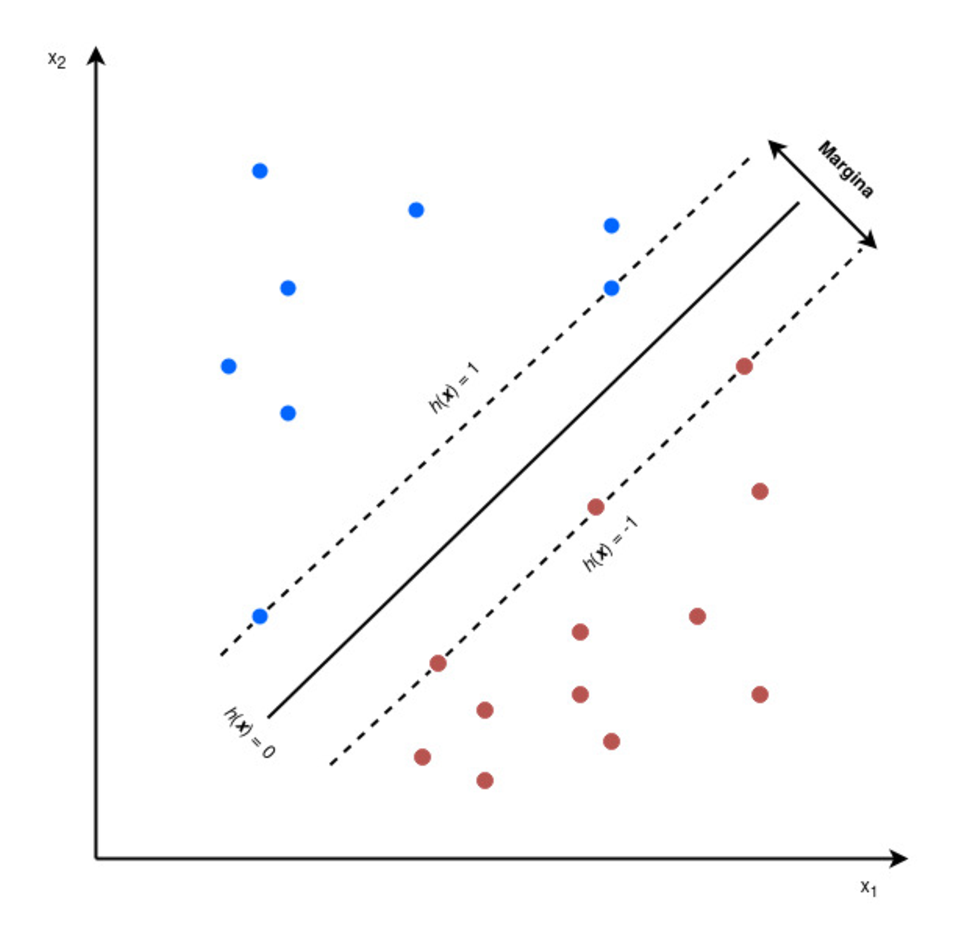
\includegraphics[width=0.65\textwidth]{svm2}
	\caption{Maksimalna margina }
	\label{svm_pic}
\end{figure}

\subsubsection{Problem višeklasne klasifikacije}

Standarnom upotrebom \gls{SVM}-model radi binarnu klasifikaciju, pa je za višeklasnu klasifikaciju $\left(K > 2\right)$ potrebno koristiti posebne metode. Osnovna ideja izvedbe jest modificirati problem višeklasne klasifikacije u više problema binarne klasifikacije. Postoji nekoliko načina na koji se ostvaruje željena modifikacija, a implementacija rješenja ma koju se rad osvrće koristi metodu jedan-naspram-ostali (engl.~\emph{one-vs-rest}) koja je zadana metoda knjižnice \emph{scikit-learn}. Princip se temelji na svođenju problema na $K - 1$ problema binarne klasifikacije, gdje je $K$ broj klasa koje početni problem može klasificirati. Tada svaki od $K-1$ binarnih klasifikatora $h_i$ odjeljuje klasu $C_i$ od svih preostalih klasa. Problem pristupa javlja se ukoliko više klasifikatora klasificira primjer kao pozitivan za svoju klasu, jer tada nije moguće jednoznačno odrediti klasu kojoj primjer pripada.

\subsection{Duboko učenje}

Duboko učenje grana je strojnog učenja čiji se modeli temelje na neuronskim mrežama \citep{cupic}. Postoji mnogo modela i varijacija, a implementacija u ovom radu koristi povratnu neuronsku mrežu (engl.~\emph{Recurrent neural network}) s arhitekturom ćelije s dugoročnom memorijom (engl.~\emph{Long short-term memory}). Ostali poznati modeli neuronskih mreža su konvulucijske neuronske mreže (engl.~\emph{Convolutional neural network}), duboke neuronske mreže (engl.~\emph{Deep neural network}), duboka probabilistička mreža (engl.~\emph{Deep belief network}). Općenito, neuronske mreže složeni su sustavi čija je osnovna gradivna jedinica neuron čiji je zadatak propuštati težinsku sumu kroz prijenosnu funkciju određujući na taj način izlaznu vrijednost. Ulazi u neuron množe se sa težinskim funkcijama $w_{1..n}$ te se sumiraju uz dodatak pomaka (engl.~\emph{bias}) $w_0$ daju vrijednost $z$ koja propuštanjem kroz prijenosnu funkciju daje izlaz $f(z)$ iz neurona. Primjer neurona prikazan je na slici \ref{neuron}.  

\begin{figure}[h]
	\centering
	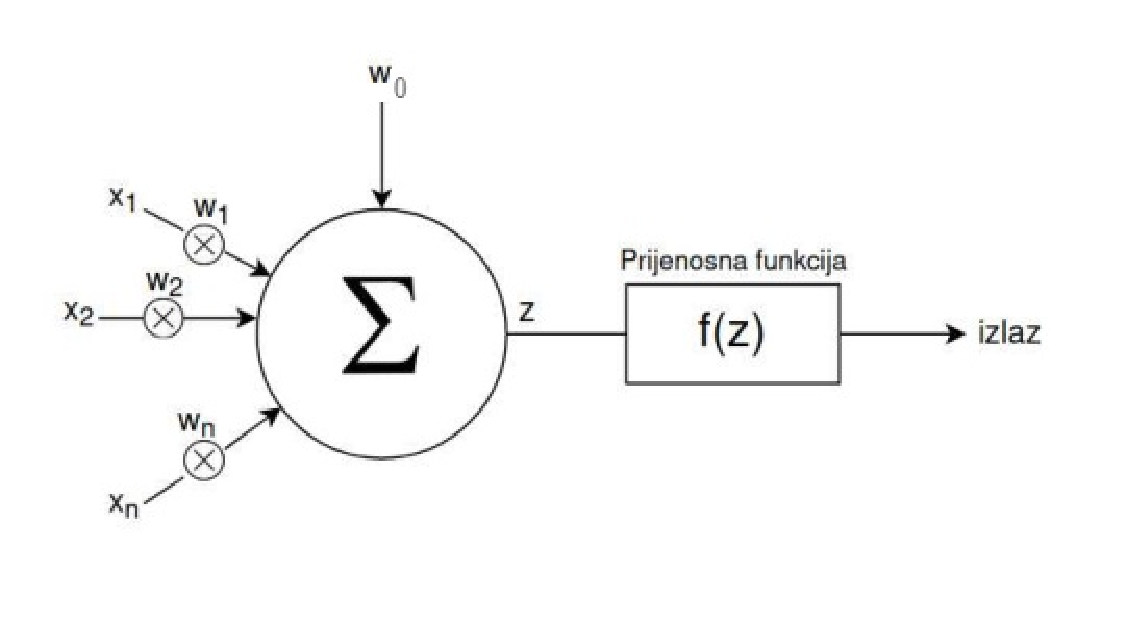
\includegraphics[width=0.75\textwidth]{neuron}
	\caption{Umjetni neuron}
	\label{neuron}
\end{figure}

\subsubsection{Prijenosne funkcije}

Propusne funkcije mogu biti razne, a najčešće su sljedeće:
\begin{itemize}
	\item binarna step funkcija $f(x)=\left\{\begin{array}{l}0 \text { for } x<0 \\1 \text { for } x \geq 0\end{array}\right.$
	\item sigmoidalna funkcija $\sigma(x)=\frac{1}{1+e^{-x}}$
	\item ReLU funkcija $max(0,x)$
	\item tanges hiperbolički funkcija $\tanh(x)$
\end{itemize}
Linearno ponašanje nije karakteristično za prirodne pojave, pa stoga linearne prijenosne funkcije nisu pogodne za upotrebu u područjima poput računalnog vida ili obrade prirodnog jezika. Nelinearne funkcije omogućuju bolju procjenu prirodnih fenomena kao što jest jezik. Najkorištenije nelinearne funkcije su sigmoidalna funkcija, tanges funkcija i \emph{ReLU} funkcija. Sigmoidalna funkcija (slika \ref{aktivacijske}(a)) najćešće je korištena funkcija izlaznog sloja kada se radi o binarnoj klasifikaciji jer skuplja sve vrijednosti na interval $[0,1]$. Slična tome je i hiperbolička tanges funkcija (slika \ref{aktivacijske}(b)) koja radi na intervalu $[-1,1]$, ali zbog svoje derivacije pruža snažniji gradijent i možemo ju smatrati superiornijom u odnosu na sigmoidalnu funkciju \citep{akt}. Funkcija koja je najćešće prisutna u \gls{LSTM} arhitekturi \gls{RNN}-a je \emph{ReLU} prijenosna funkcija (slika \ref{aktivacijske}(c)) koja svim negativnim vrijednostima pridaje vrijednost 0, dok pozitivne vrijednosti slijede linearnu funkciju. Postoji varijacija te aktivacijske funkcije po imenu \emph{Leaky ReLU} koja za negativne vrijednosti slijedi funkciju $f(x) = 0.01x$, a za pozitivne se ponaša isto kao \emph{ReLu} i slijedi funkciju $f(x) = x$ ili eventualno $f(x) = kx$.

\begin{figure}
     \centering
     \subfloat[][sigmoidalna funkcija]{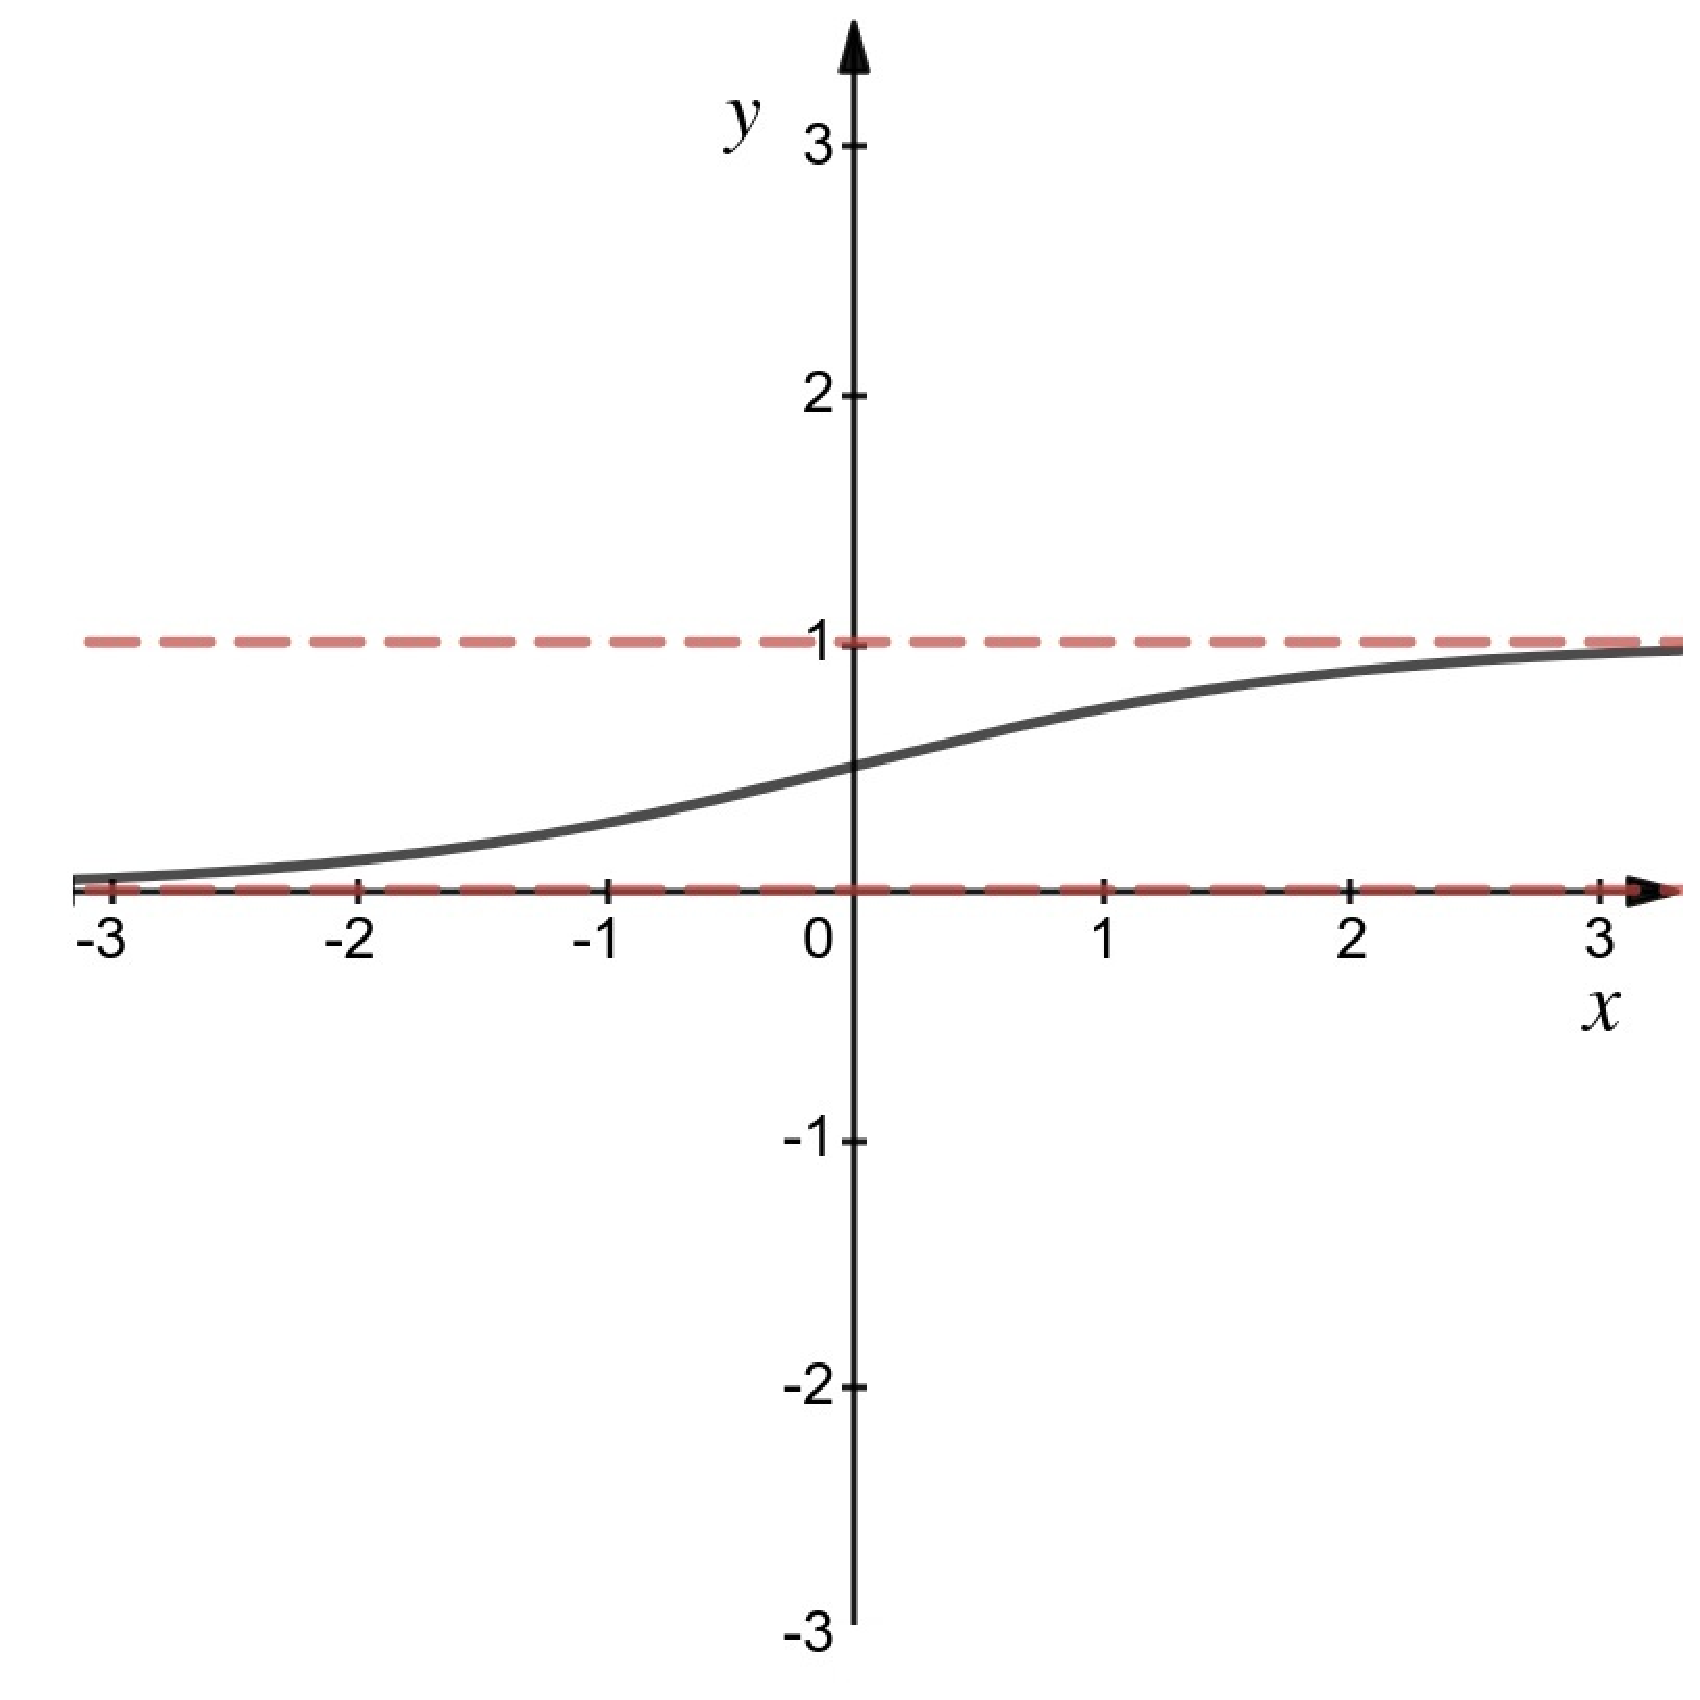
\includegraphics[width=0.2\textwidth]{sigm}\label{sigm}\hspace{7mm}}
     \subfloat[][tanh(x)]{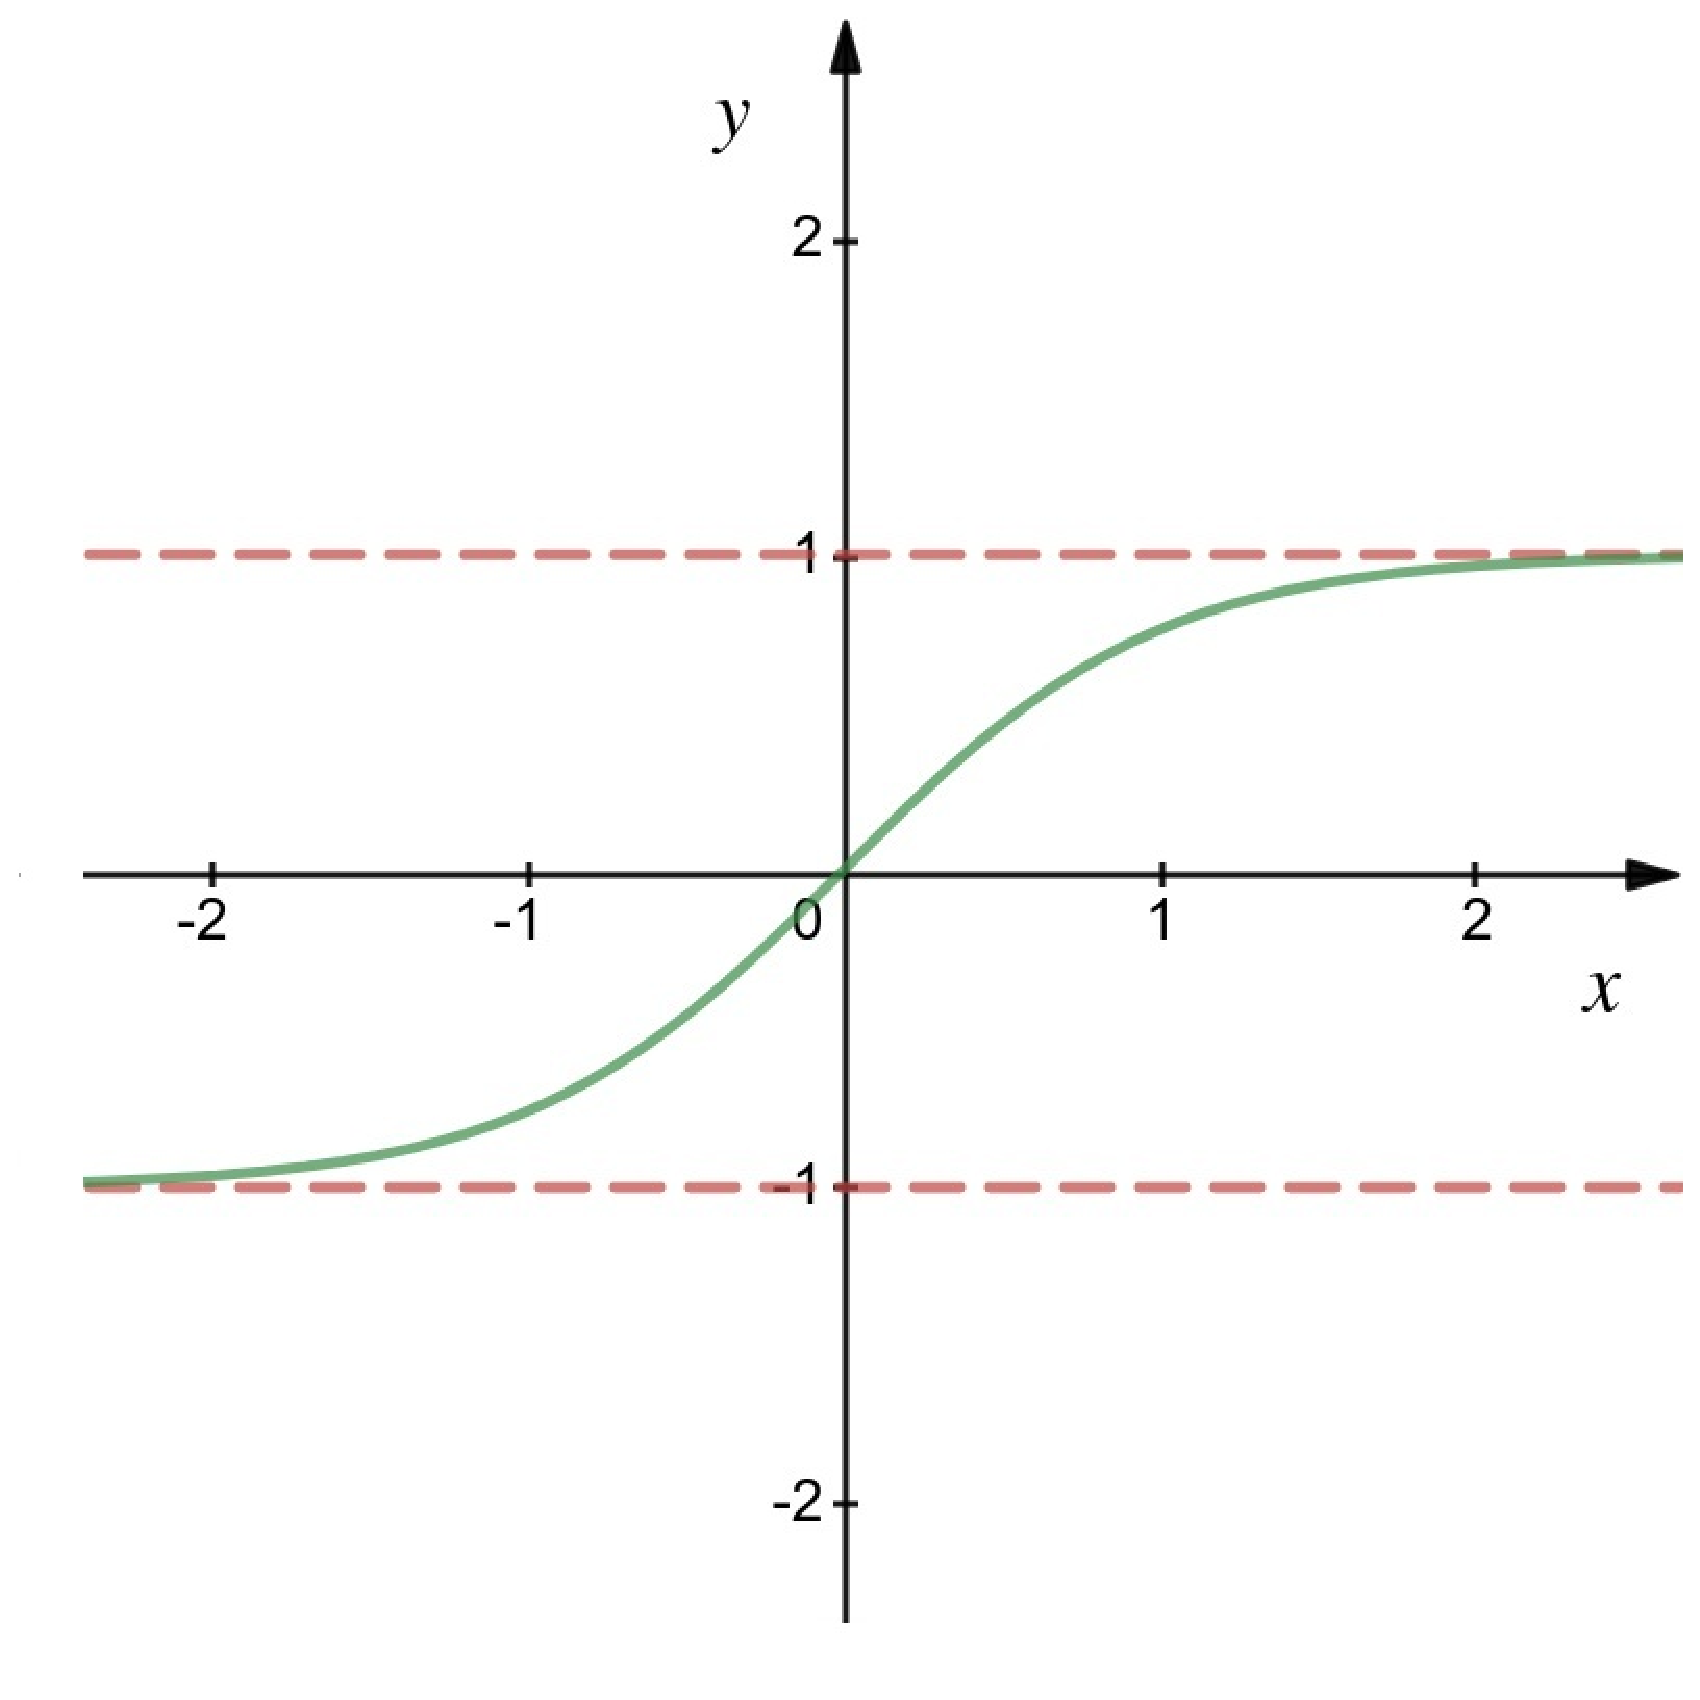
\includegraphics[width=0.2\textwidth]{tanh}\label{tanh}\hspace{7mm}}
     \subfloat[][\emph{ReLU}]{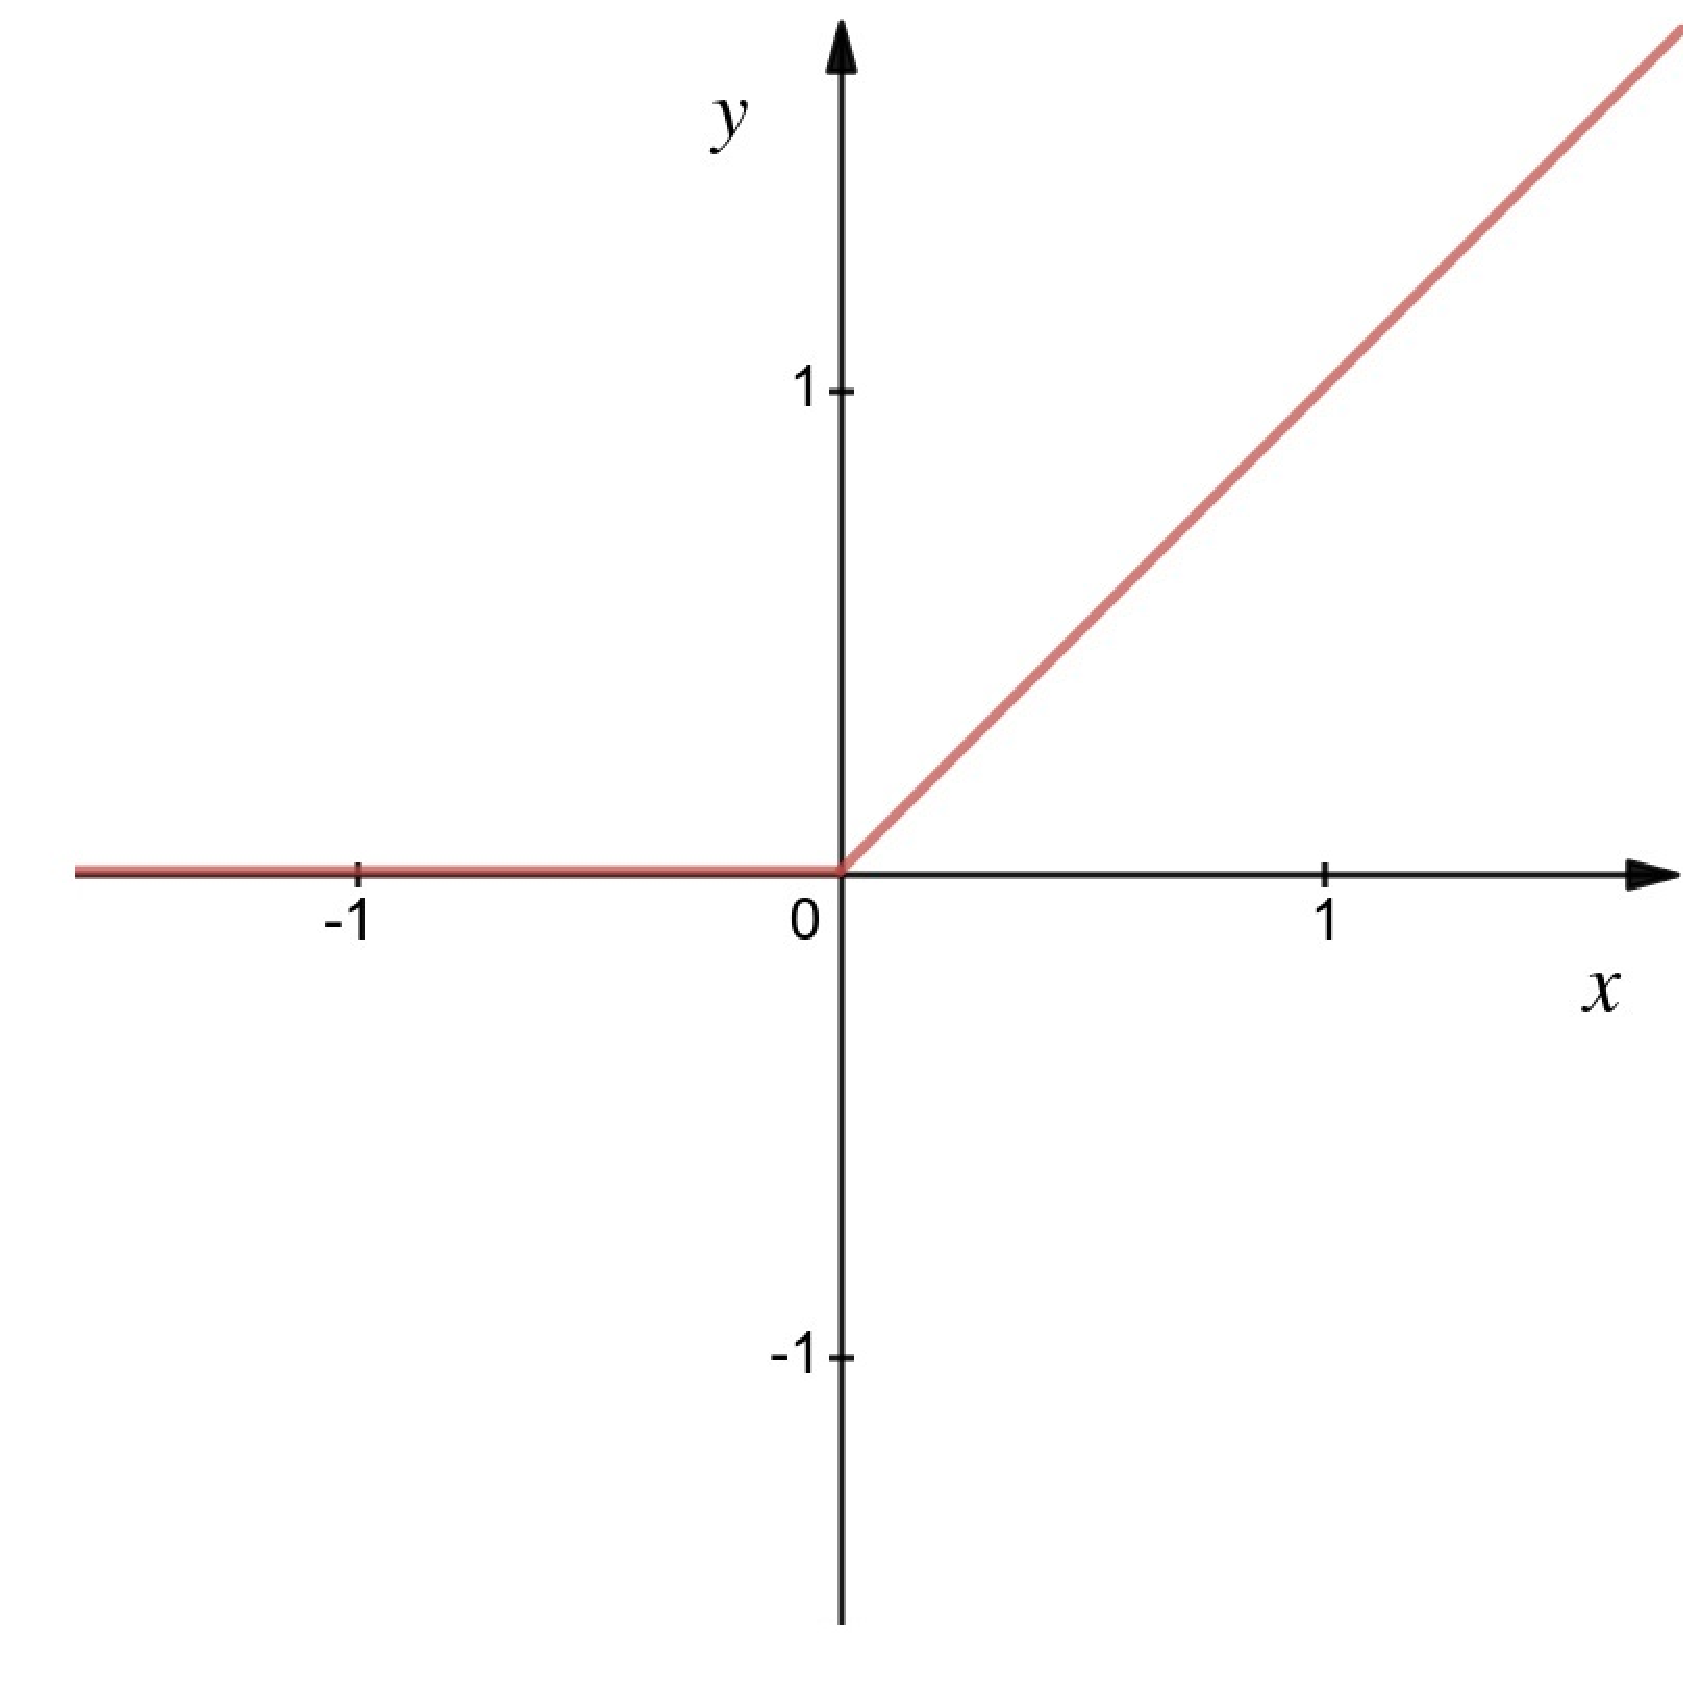
\includegraphics[width=0.2\textwidth]{relu}\label{relu}}
     \caption{Aktivacijske funkcije}
     \label{aktivacijske}
\end{figure}

\subsubsection{Povratne neuronske mreže}
Arhitektura mreže koja je implementirana u radu je povratna neuronska mreža (\gls{RNN}) koja pripada porodici slojevitih unaprijednih neuronskih mreža. To znači da u sebi nema cikluse, odnosno ulazi neurona ne ovise o izlazima neurona koji se nalaze u dubljim slojevima. Karakteristika povratne neuronske mreže prisutnost je memorije. To im omogućeje obradu sekvencionalnih ulaza, odnosno mreže takvih arhitektura uzimaju u obzir poredak ulaznih podataka i time stvaraju povezanost između ulaza. Princip rada može se objasniti uz pomoć prikaza na slici \ref{rnnprincip}. Za ulaz $x_0$ u prvom koraku vrijedi da je ulaz jednak $x_0$, a za svaki sljedeći ulaz vrijedi da je jednak $x_{t} + h_{t-1}$, odnosno kombinaciji izlaza iz prethodnog koraka i trenutnog ulaza iz skupa ulaznih podataka. Problem koji se javlja u RNN-arhitekturi jest takozvani gubitak gradijenta, odnosno događa se da vrijednost u neuronu postaje toliko beznačajna da je daljnje treniranje gotovo onemogućeno \citep{rnn_training}. Tome se doskače korištenjem ćelije s dugoročnom memorijom (\gls{LSTM}).

\begin{figure}
	\centering
	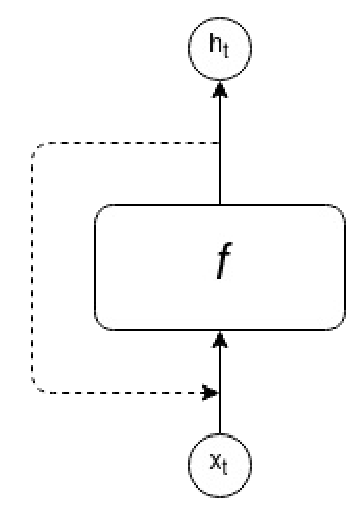
\includegraphics[width=0.3\textwidth]{rnn}
	\caption{Princip ponašanja povratne neuronske mreže}
	\label{rnnprincip}
\end{figure}

\subsubsection{Arhitektura ćelije s dugoročnom memorijom}
Arhitektura ćelije s dugoročnom memorijom (\gls{LSTM}) prikazana je na slici \ref{lstmarh}. Sastoji se od triju ulaznih vrata:
\begin{itemize}
	\item ulazna vrata
	\item vrata za zaboravljanje
	\item izlazna vrata
\end{itemize}

Ulazna vrata odgovorna su za odabir vrijednosti koje će modificirati stanje u memoriji. Sastoje se od sigmoidalne i tanges hiperbolične funkcije. Sigmoidalna funkcija odgovorna je za odabir vrijednosti koje će sudjelovati u modifikaciji memorije, a tanges hiperbolični odgovoran je za pridjeljivanje odgovarajuće težine ulazu. Vrata za zaboravljanje odgovorna su za prebiranje vrijednosti iz prethodne iteracije i ulaznog podatka i također funkciniraju na temelju sigmoidalne funkcije. Izlazna vrata određuju izlaz koristeći ulazni podatak i stanje u memoriji, a kada je riječ o prijenosnim funkcijama izvedba im je jedanaka ulaznim vratima. Funkcionalnost \gls{LSTM} arhitekture zapisana jednadžbama je sljedeća: \[ \begin{aligned}
f_{t} &=\sigma_{g}\left(W_{f} x_{t}+U_{f} h_{t-1}+b_{f}\right) \\
i_{t} &=\sigma_{g}\left(W_{i} x_{t}+U_{i} h_{t-1}+b_{i}\right) \\
o_{t} &=\sigma_{g}\left(W_{o} x_{t}+U_{o} h_{t-1}+b_{o}\right) \\
\tilde{c}_{t} &=\sigma_{h}\left(W_{c} x_{t}+U_{c} h_{t-1}+b_{c}\right) \\
c_{t} &=f_{t} \circ c_{t-1}+i_{t} \circ \tilde{c}_{t} \\
h_{t} &=o_{t} \circ \sigma_{h}\left(c_{t}\right)
\end{aligned}, \]
gdje je $x_t$ vektor ulaznih podataka, $f_t$ aktivacijski vektor vrata za zaborav, $o_t$ aktivacijski vektor izlanih vrata, $i_t$ aktivacijski vektor ulaznih vrata, $h_t$ izlazni vektor \gls{LSTM}-a, $\tilde{c}_t$ aktivacijski vektor ulaza u ćeliju, $c_t$ vektor stanja ćelije i konačno $W, U$ i $b$ matrice težina i pomaka koje je potrebno naučiti tjekom treniranja.

\begin{figure}[h]
	\centering
	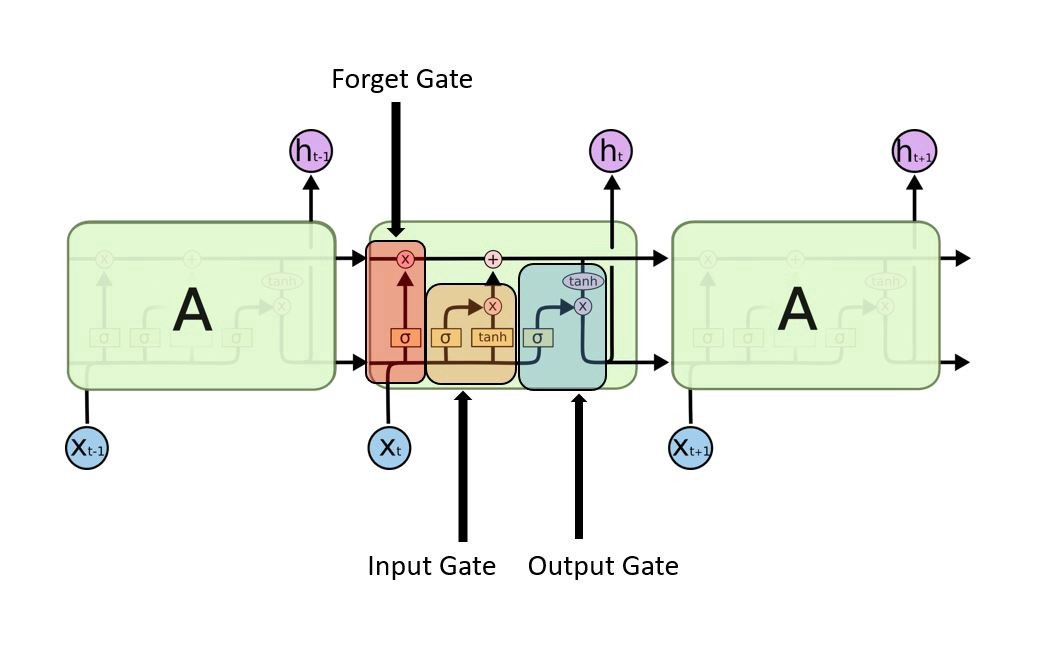
\includegraphics[width=0.65\textwidth]{lstm}
	\caption{\gls{LSTM} arhitektura}
	\label{lstmarh}
\end{figure}



\section{Obrada ulaznih podataka}

Zbog prirode mikroblogova ulazni su podatci prošarani raznim značajkama koje je potrebno ukloniti ili preinačiti. Pri stvaranju podataka pogodnih za izradu značajki nastale su dvije vrste podataka.\\
\noindent Prva je jednostavna i služi izradi značajki temeljenih na frekvencijama riječi ili vektorima riječi. Dobivena je tako što je prvo provedena zamijena emotikona s njihovom jezičnom reprezentacijom u smislu da je npr.~":-)" pretvoreno u \emph{"happy"}. Zatim je provedeno uklanjanje svih nejezičnih elemenata kao što su hiperlinkovi, korisnička imena, emotikoni, brojevi i slično. Mikroblogovi su rastavljeni na riječi koristeći biblioteku \emph{Spacy} te je nad dobivenim skupom jezičnih elemenata proveden postupak ispravljanja pravopisa i prepoznavanje žargona. Uklonjene su riječi koje ne doprinose značenju. Takve se riječi nazivaju zaustavne riječi (engl.~\emph{stop-words}) i uklonjene su koristeći biblioteku za obradu prirodnog jezika \emph{Natural Language Toolkit (NLTK)} \citep{nltk}. Na preostalim riječima proveden je postupak lematiziranja, odnosno pretvaranja riječi iz izvedenog oblika u njen korijenski oblik, takozvanu lemu. Za postupak lematiziranja korišten je \texttt{WordNetLemmatizer} iz spomenute biblioteke \gls{NLTK}.\\
\noindent Druga vrsta sastoji se od mikroblogova koji su označeni koristeći alat koji je napravio spomenuti tim \emph{DataStories} s natjecanja \emph{Semeval} \citep{datastories-Semeval}. U mikroblogu se ovim postupkom označavaju elementi poput hiperlinkova, cenzuriranih riječi, brojeva, riječi napisanih velikim slovima, korisničkih imena i slično. Takve su podatci ostavljeni u obliku teksta, odnosno nisu razlomljeni na manje elemente, jer su korišteni za prebrojavanje prisutnosti spomenutih elemenata.

\section{Značajke}

S obzirom na to da se paralelno koriste dva pristupa izrade i treninga modela, izrada i korištenje značajki također je podijeljena u dva smjera. Izrada značajki za klasično strojno učenje znatno je opsežniji i kreativniji proces nego izrada istih za pristup dubokim učenjem. Moglo bi se reći da je srž klasičnog pristupa upravo u izradi značajki jer se modeli sami po sebi ne mogu značajno konfigurirati, pa rezultat najviše ovisi o onome što mu se na ulazu pruži. Kod dubokog učenja postoje jednostavni standardni pristupi koji su ponekad gotovo mandatorni. 


\subsection{Značajke u klasičnom pristupu}

Značajke u ovom pristupu čine glavnu okosnicu uspjeha modela, pa je stoga izradi posvećen znatan udio vremena. Značajke se mogu grupirati u tri kategorije: \begin{itemize}
\item brojanje riječi i vektori riječi
\item polaritet i sentiment riječi
\item brojanje prisutnosti elemenata
\end{itemize}

\subsubsection{Brojanje riječi i vektori riječi}

U ovoj se kategoriji nalaze dvije vrste značajki koje se međusobno isključuju, odnosno ne koriste se istovremeno. Prva značajka je uobičajena kao početni uzorak značajki koji se koristi za treniranje osnovnog modela (engl.~\emph{baseline model}) kao referenca za daljnje eksperimente. Radi se 
se o metodi vreće riječi (engl. \emph{Bag-of-Words}), odnosno preciznije o primjeni mjere učestalosti riječi \emph{TF-IDF} (engl. \emph{term  frequency-inverse  document  frequency}). Mjera se definira na sljedeći način: potrebno je definirati dvije zasebne statističke mjere -- mjeru učestalosti izraza (\emph{tf}) i inverznu učestalost u dokumentima (\emph{idf}). Prvu mjeru koja označava učestalost pojave riječi računamo na sljedeći način: \[ \mathrm{tf}(t,d) = 0.5 + 0.5 \cdot  \frac{f_{t, d}}{\max\{f_{t', d}:t' \in d\}}\]
\noindent\\
gdje $t$ predstavlja izraz, $d$ predstavlja dokument, odnosno skup svih izraza u promatranom tekstu, $f_{t,d}$ predstavlja broj pojavljivanja izraza u tekstu, a brojnik predstavlja neveći broj pojavljivanja nekog izraza u tekstu. Ova se normalizirana verzija učestalosti pojave izraza koristi radi sprječavanja pristranosti prema velikim tekstovima.
Druga mjera koju određujemo je inverzna učestalost izraza u dokumentu i računa se na sljedeći način:
\[ \mathrm{idf}(t, D) =  \log \frac{N}{|\{d \in D: t \in d\}|} \]
\noindent\\
gdje $D$ predstavlja skup svih tekstova na kojima računamo učestalost, a nazicnik razlomka predstavlja broj pojavljivanja izraza u tekstu, dok je $N$ ukupan broj dokumenata u skupu $D$.
Konačna mjera jednaka je umnošku dviju prethodno izračunatih mjera, odnosno: \[ {\displaystyle \mathrm {tfidf} (t,d,D)=\mathrm {tf} (t,d)\cdot \mathrm {idf} (t,D)} \]
\noindent
U implementaciji rješenja koristim gotovu metodu iz knjižnice \emph{scikit-learn}. Korištenjem nastalih značajki u \gls{SVM}-modelu dobio sam točnost od $39.5\%$, što je korektan osnovni model s obzirom na točnost nasumičnog odabira koja iznosi $33.3\%$.\\\\
Druga značajka koju sam uveo, a koja pripada ovoj kategoriji, temelji se na vektorima riječi iz knjižnice \emph{Spacy}. Radi se o vektorima s 300 dimenzija nastalima primjenom \emph{Word2vec} \citep{w2v} metode. \emph{Word2vec} je model plitke neuronske mreže s dva sloja koji treniranjem pokušava rekonstruirati lingvističko značenje riječi. Kao ulaz koristi vrlo velik skup tekstualnih podataka koji mogu biti raznog porijekla, kao npr.~ članci \emph{Wkipedie}, objave na društvenim mrežama, primjerci elektroničke pošte itd.~Kao rezultat nastaju višedimenzionalni vektori čije se dimenzije obično kreću između $100$ i $1000$ dimenzija. Vektori su u prostoru smješteni na način da su vektori riječi bliskog znanja prostorno bliski jedan drugome.\\
Koristeći prethodno izrađene informacije proizašle iz metode \emph{tf-idf} kodirao sam ulazne informacije vektorima riječi na način da sam izračunao prosječnu vrijednost vektora svih riječi koje se pojavljuju u mikroblogu, a za broj značajki u tako nastalom vektoru odabrao sam vrijednost broja riječi u najduljem mikroblogu. Poboljšanje nastalo korištenjem ovih značajki značajno je povečalo uspješnost modela koji je nakon treniranja imao točnost od $60.9\%$

\subsubsection{Polaritet i sentiment riječi}

S obzirom na to da je zadatak klasifikacija s obzirom na polaritet mikrobloga, bilo je nužno dotaknuti se polariteta i sentimenta samih riječi. Za to su iskorištena dva leksikona. Prvi od njih je leksikon ocjena riječi koji sadrži ocjene po atributima zadovoljstva, uzbuđenosti i dominantnosti po imenu  \emph{Affective Norms for English Words} \citep{anew}. Prva verzija sastojala se od nešto više od tisući riječi, no 2013. godine proširena je na $14000$ \citep{anew2}. Pri implementaciji rješenja korišten je pristup temeljen na pristupu koji je prisutan u repozitoriju \emph{dwzhou/SentimentAnalysis} \citep{anew_code}. Drugi leksikon koji je korišten je zapravo običan popis pozitivnih i negativnih riječi \citep{leksikon}. 
\noindent Dodavanjem značajki dobivenih korištenjem leksikona podigao sam točnost modela za $1\%$, odnosno postigao točnost od $61.9\%$.

\subsubsection{Brojanje prisutnosti elemenata}

U ovoj se kategoriji nalaze značajke nastale brojanjem ili promatranjem prisutnosti raznih elemenata u mikroblogovima. Elementi čija je prisutnost naznačavana zastavicama $0$ ili $1$ su: \emph{e-mail} adrese, hiperlinkovi, znakovi valute, datumi, telefonski brojevi itd.~Za neke se elemente bilježio točan broj pojavljivanja u mikroblogu, a izrazi za koje je bilježena ta informaciju su: izrazi s nizanjem znakova (npr.~\emph{"cooool"}), izrazi napisani velikim slovima, cenzurirani izrazi (npr.~\emph{"F***}), broj ponovljenih riječi, pojave takozvanih \emph{hashtagova} i broj uskličnika. Kao dodatna značajka nadodan je i ukupan broj riječi u rečenici.
\noindent Dodavanjem ovih značajki ostvaren je porast točnosti od $0.4\%$, odnosno postignuta je konačna točnost \gls{SVM}-modela od $62.32\%$.

\subsection{Značajke u dubokom učenju}

Izrada značajki korištenih u modelu dubokog učenja znatno je jednostavnija. Potrebno je izgraditi vokabular riječi koje se pojavljuju u skupu podataka i svakoj riječi u vokabularu pridjeliti redni broj koji će služiti kao oznaka riječi. Zatim je potrebno izgraditi matricu vektora riječi (engl.~\emph{embedding matrix}) koja se sastoji od onoliko stupaca koliko vektor riječi ima dimenzija, što je u slučaju ove implementacije 300 dimenzija. U redovima su po rednim brojevima iz vokabulara kodirane riječi odgovarajučim vektorima riječi. Model tjekom inicijalizacije prima matricu vektora. Pomoću izrađenog vokabulara vrši se kodiranje sadržaja mikroblogova, odnosno umjesto tekstualnog sadržaja mikroblogovi postaju vektori brojeva koji predstavljaju redni broj riječi u vokabularu. Radi konzistentnosti dimenzija odabrana je maksimalna veličina vektora koja odgovara najvećem vektoru u skupu podataka za treniranje, a svi manji vektori nadopunjavaju se nulama do željene veličine. Takav skup vektora predaje se modelu kao ulaz u treningu i u evaluaciji modela.

\chapter{Provedba eksperimenata}

Ovo poglavlje opisuje proces provođenja eksperimenata i osvrće se na postignute rezultate. Detaljno opisuje karakteristike implementacija i uspoređuje učinke izmjena modela koje su se činile tijekom eksperimentiranja, kao i podešavanje hiperparametara.

\section{Podatci}

Skup podataka za trening sastoji se od $49491$ mikroblogova, dok se skup podataka za testiranje sastoji od $12258$ mikroblogova. Podatci su odmah podijeljeni na one za treniranje i one za testiranje jer je sam skup podataka proizašao iz natjecanja \emph{Semeval 2017}, pa su korišteni originalni podatci za odgovarajuće faze natjecanja, tako da su rezultati postignuti na testnom skupu podataka mjerodavni onima koji su dobiveni kao rezultati natjecanja. Podatci se strukturno sastoje od identifikacijskih brojeva objava, oznake polariteta objave i teksta objave. Identifikacijske oznake izbačene su prilikom učitavanja jer niti jedna značajka ne proizlazi iz njih. 
Primjer jedne originalne objave:\\\\
\texttt{
"(OFF TOPIC) - there is only 3 episodes on the first disk of \#Dexter. Please hurry, @netflix with the 2nd \#fitblog" 
}

Ti su podatci obradom poprimili oblik prikladan izvlačenju značajki, pa je prethodno spomenuta objava pretvorena u dvije vrste podataka. Prva vrsta jest popis riječi koje se nalaze u objavi, a koje ne pripadaju zaustavnim riječim (enlg.~\emph{stop-words}).


\chapter{Zaključak}

%TODO

\bibliography{literatura}
\bibliographystyle{fer}
\printglossaries

\begin{sazetak}
Ovaj se rad bavi analizom sentimenta u mikroblogovima društvene platforme \emph{Twitter}. Proučavanje teme analize sentimenta ostvareno je uz pomoć četvrtoga zadatka s najtecanja \emph{Semeval} koji je bio vrlo popularan zadatak nekoliko godina u nizu u kojima se natjecanje održavalo. Napravljena je usporedba pristupa klasičnim strojnim učenjem, odnosno korištenja \gls{SVM}-modela i pristupa dubokog učenja, odnosno korištenja povratne neuronske mreže (\gls{RNN}) s arhitekturom ćelije s dugoročnom memorijom (\gls{LSTM}). S pristupom klasičnog strojnog učenja ostvarena je točnost od $62.3\%$, a pristupom dubokog učenja osvarena je nešto bolja točnost od $64\%$, što implementaciju stavlja na 11. mjesto implementacija koje su bile predane u sklopu natjecanja 2017. godine.

\kljucnerijeci{strojno učenje, duboko učenje, obrada prirodnog jezika, analiza sentimenta, analiza mikroblogova, Semeval} 
\end{sazetak}

The theme of this thesis is sentiment analysis on microblogs from the social platform \emph{Twitter}. %TODO

\engtitle{Machine Learning for Sentiment Analysis in Microblogs}
\begin{abstract}
Abstract.

\keywords{Machine learning, Deep learning, Natural language processing, Sentiment analysis, Microblogs analysis, Semeval.}
\end{abstract}


\end{document}
